\documentclass[conference]{IEEEtran}
\usepackage{graphicx}
\usepackage{amsmath}
\usepackage{booktabs}
\usepackage{array}
\usepackage{cite}
\usepackage{url}
\usepackage[hidelinks]{hyperref}
\renewcommand{\topfraction}{0.9}
\renewcommand{\dbltopfraction}{0.9}
\renewcommand{\textfraction}{0.07}
\renewcommand{\floatpagefraction}{0.85}
\renewcommand{\dblfloatpagefraction}{0.85}
\setcounter{dbltopnumber}{2}
\begin{document}
\bstctlcite{IEEEexample:BSTcontrol}
\title{What a Tooth-Level Caries Score Cannot Tell You:\\ An Image-Blind Floor, Measured Across Cohorts and Sites, for Panoramic Dental Radiographs}
\author{\IEEEauthorblockN{[ASK AUTHOR: author names]}
\IEEEauthorblockA{[ASK AUTHOR: affiliations and e-mail addresses]}}
\maketitle
\begin{abstract}
Systems that find dental caries on panoramic radiographs are compared by which teeth they mark as carious. Caries concentrates on a few tooth positions, so part of that score can be earned without looking at the image. We derive the F1 of the best image-blind tooth list in closed form: it holds exactly the teeth whose caries prevalence exceeds half its F1. Fitted on 78 held-out radiographs, the rule returns the eight first and second molars, which score F1 0.320 on our 164 scored images. Against this floor we scored a six-stage pipeline with two interchangeable caries stages and two vision-language models, on development data, four external sites and a public benchmark. Both language models scored below the floor. A per-tooth crop classifier led the floor on development data but was level with it on the four external sites (+0.89 points [$-$3.86, +5.57]). A whole-image lesion detector, adopted under a rule fixed before training, led it there by 9.28 points [+4.72, +13.73] while flagging fewer teeth, at three of the four sites. That cohort also informed the detector's adoption, and pooled as a sample of sites the lead's interval includes zero. On these cohorts a tooth-level score alone was not enough to tell whether a system reads the radiograph; it should be reported with an image-blind row and per-site results.
\end{abstract}
\begin{IEEEkeywords}
panoramic radiography, dental caries, image-blind baselines, shortcut learning, external validation, object detection, selective prediction
\end{IEEEkeywords}

\section{Introduction}

A panoramic dental radiograph (orthopantomogram) is one X-ray of both jaws unrolled into a wide image (Fig.~\ref{fig:1}). It is displayed as if the viewer faces the patient, so the patient's right side is on the image's left. Teeth are named in the two-digit notation of the Fédération Dentaire Internationale (FDI): the first digit is the quadrant (1 upper right, 2 upper left, 3 lower left, 4 lower right, in the patient's frame) and the second the position counted from the midline (1 central incisor to 8 third molar). Tooth 36 is the lower-left first molar. Caries dissolves mineral, so a lesion appears as a darker region inside the bright tooth.

\begin{figure*}[t]
\centering
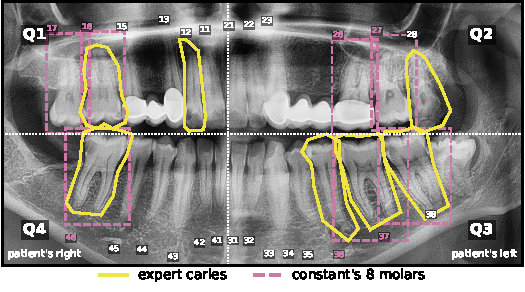
\includegraphics[width=0.86\textwidth]{figures/R01_opg_primer.pdf}
\caption{Reading a panoramic radiograph. One held-out DENTEX radiograph (test\_120) cropped to the teeth. Dotted lines separate the quadrants; numbers are the FDI codes our numbering stage assigned. Yellow: the expert's seven caries annotations as released. Dashed: the eight-molar set \{16, 17, 26, 27, 36, 37, 46, 47\} named by the image-blind list of Section III-B; seven of its codes are present here and four of the seven lesions lie on them. Radiograph: DENTEX~\cite{hamamci2023dentex}, CC BY-NC-SA 4.0.}
\label{fig:1}
\end{figure*}

Automated caries systems are usually compared by which teeth they mark as carious, and a high tooth-level score is read as evidence that a system sees the lesions. Our motivation is that this reading can fail: caries is not spread evenly over the mouth, and in our data the first and second molars carry most of it, so a list of molars chosen without any image already earns much of the score, and a high score alone does not distinguish a system that reads the image from one that has learned where caries usually is. A learner that minimises error over a population will use any cue that predicts the label, and position predicts it: a shortcut~\cite{geirhos2020shortcut}.

Other fields test for this with baselines that withhold the input the task is about, in natural-language inference and chest radiography~\cite{poliak2018hypothesis,zech2018variable}, or by rebalancing the data so that a prior no longer pays, in visual question answering~\cite{goyal2017making}. We found no such baseline in the dental papers we surveyed; this is an observation from our reading, not a systematic count. External validation is also uncommon in medical-imaging artificial intelligence~\cite{kim2019design}.

We therefore ask three questions. RQ1: does tooth-level agreement separate a full pipeline from an image-blind list, on development data and on external cohorts? RQ2: does recasting the caries stage from classifying tooth crops to localising lesions in the whole image, a task a fixed list cannot perform, separate them? RQ3: what does the pipeline show on outputs a fixed list cannot produce?

Our approach is to give the floor in closed form, so that it can be computed from label prevalence alone and checked against saved scores, and to measure every system against it. The pipeline is modular because no public dataset labels teeth, caries and other findings together, so each stage is trained on the dataset that carries its label and the stages are joined on the FDI code. Two rules of the evaluation are also the authors' choices: the lesion detector's adoption rule was fixed before training, so that its comparison with the image-blind list could not be tuned afterwards, and the tooth detector, adopted against its registered guard, is reported as a decision taken against that rule. The contributions are:

\begin{enumerate}
\item A short account of the tooth-level caries score: the closed-form F1 of an image-blind list and the rule that selects it, the dependence of lesion agreement on each cohort's prior, and a test for a positional shortcut, each set against our data (Section III).
\item The floor measured on three cohorts and four external sites with paired intervals: eight molars at F1 0.320, which a crop classifier led only on its development data (Section VI-A).
\item A pre-registered recasting of the caries stage as lesion detection, which led the floor on the pooled external sites with fewer flagged teeth, and the evidence for and against reading it as perception (Section VI-B).
\end{enumerate}

Section II places the work; Section III gives the account; Sections IV and V describe the system, data and protocol; Section VI answers the three questions; Section VII discusses what follows for reporting, and Section VIII bounds it.

\section{Related Work}

\textbf{Shortcuts and input-blind baselines.} Shortcut learning describes models that exploit any cue correlated with the label~\cite{geirhos2020shortcut}. Fields that recognised this built controls for it. Visual-question-answering models were found, on data rebalanced with complementary image pairs, to have answered from language priors while ignoring the image~\cite{goyal2017making}, and lost accuracy when answer priors changed between training and test~\cite{agrawal2018dont}. In natural-language inference, a model that never sees the premise beats the majority class on many datasets~\cite{poliak2018hypothesis}. In medical imaging, COVID-19 detectors relied on confounders and failed at new hospitals~\cite{degrave2021ai}, and in a pneumonia task the hospital alone reached an area under the ROC curve (AUC) of 0.861 because prevalence differed between sites~\cite{zech2018variable}. Averages can also hide subgroups on which a model fails~\cite{oakdenrayner2020hidden}. Our contribution is to bring such a floor to tooth-level caries scoring, give it a closed form and measure it across cohorts and sites.

\textbf{Dental caries analysis and transfer.} We use the Tufts Dental Database of 1,000 radiographs~\cite{panetta2022tufts}, DENTEX with quadrant, enumeration and diagnosis labels~\cite{hamamci2023dentex}, the CariesXrays benchmark of 6,000 radiographs~\cite{chen2024cariesxrays}, the multi-centre dataset of Li et al., which the authors describe as collected at three hospitals~\cite{li2024multicenter}, and UFBA-425~\cite{budagam2024oralbbnet}. A systematic review found accuracies of 86.1 to 96.1\% for caries classification models on panoramic radiographs, and judged the quality and reporting of the studies it reviewed to be low~\cite{mohammadrahimi2022deep}. Caries and related analysis has used dual networks~\cite{lim2024dual}, dedicated convolutional classifiers~\cite{bilal2024pdcnet} and contrastive feature pyramids~\cite{chen2024cariesxrays}. Numbering is reported at very high figures when teeth are classified from crops, for example a class-averaged accuracy of 0.9988~\cite{zancan2025ai}, and multi-stage systems number teeth on Tufts and other datasets~\cite{zhang2025reliable}; numbering under detector output is harder, because teeth can be missed or duplicated. Of 516 eligible medical-imaging AI studies published in 2018, 31 validated externally~\cite{kim2019design}. Dental models tested on other data lose accuracy: an apical-lesion model fell from F1 54.1\% to 32.7\% at a second centre~\cite{krois2021generalizability}, and a YOLOv11 detector of 13 conditions fell from mAP@0.5 0.857 to 0.806 on externally collected web images, with lower performance on subtle findings such as bone loss and caries~\cite{mutlu2026comparison}. One enumeration-then-caries detector reported lesion sensitivity of 0.70 internally and 0.67 externally, with patient-level specificity of 0.44 and 0.42~\cite{bizjak2024advancing}.

\section{What a Tooth-Level Score Measures}

\subsection{The report as a chain of decisions}

A report's entry for a tooth is correct only if the tooth is detected ($D$), numbered correctly once detected ($N$), and given the right finding ($F$):

\begin{equation}
P(\text{entry correct}) = P(D)\, P(N \mid D)\, P(F \mid D, N).
\end{equation}

The first two factors concern identity, not disease, and bound everything after them: a perfect caries model still writes a wrong report on a tooth that was missed or misnumbered. A metric that matches findings to teeth by code charges for both factors; one that matches lesions by position in the image is blind to the second. Table~\ref{tab:1} gives our pipeline's identity factors: on DENTEX, whose other images trained the detector, 92.8\% of teeth survive both; on UFBA-425, which no model trained on, 44.5\% do as the files are distributed.

\begin{table}[t]
\centering
\caption{Identity before disease: the first two factors of (1) per tooth, in percent, with a 95\% cluster-bootstrap interval for their product. DENTEX 164 images; Tufts test 143; UFBA-425 425, as distributed and widened to a panoramic shape.}
\label{tab:1}
\footnotesize
\setlength{\tabcolsep}{3pt}
\begin{tabular}{>{\raggedright\arraybackslash}p{1.65cm}rrrr}
\toprule
Corpus & Teeth & Detected & Exact, of detected & End to end \\
\midrule
DENTEX & 936 & 99.6 & 93.2 & 92.8 [90.6, 94.9] \\
Tufts test & 3,760 & 89.3 & 71.1 & 63.5 [59.3, 67.5] \\
UFBA-425 as is & 11,591 & 66.6 & 66.8 & 44.5 [42.4, 46.6] \\
UFBA-425 widened & 11,591 & 95.6 & 80.8 & 77.2 [75.2, 79.1] \\
\bottomrule
\end{tabular}
\end{table}

\subsection{The best image-blind list, in closed form}

Let $N$ images be scored, $P$ be the number of carious teeth over all of them, and $n_c$ the number of images in which tooth code $c$ is carious, so that $p_c = n_c/N$ is the prevalence of caries at position $c$. A constant names the same set $S$ of codes for every image. Its true positives are $\sum_{c \in S} n_c$ and it names $|S|N$ codes, so its micro-averaged F1 over teeth (FDI-set F1) is

\begin{equation}
F_1(S) = \frac{2 \sum_{c \in S} n_c}{|S|\,N + P}.
\end{equation}

Equation (2) counts every named code as a prediction, present tooth or not, as our scorer does, and applies to any set prediction scored by micro-F1 over a fixed label set. Writing $A = \sum_{c \in S} n_c$ and $k = |S|$, adding a code $c \notin S$ raises the score if and only if

\begin{equation}
p_c > \tfrac{1}{2}\, F_1(S).
\end{equation}

For a fixed size the best set is the $k$ most prevalent codes. Along this ordering F1 rises to a single peak: if code $k+1$ fails (3) against the first $k$, every later, less prevalent code fails too. The best constant therefore holds exactly the codes with $p_c > \tfrac{1}{2}F_1^{*}$: a functional of the caries prior alone. That first molars are the most caries-susceptible teeth has long been reported, for example in a large longitudinal study of children~\cite{batchelor2004grouping}; the prior, and with it the floor, depends on the population.

\begin{figure*}[t]
\centering
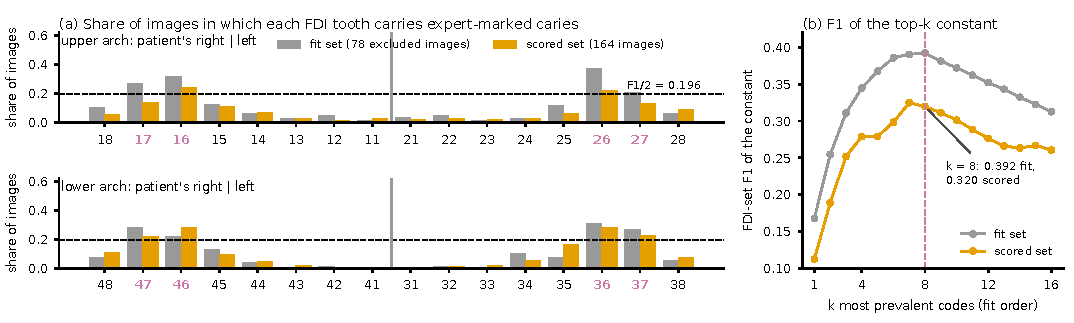
\includegraphics[width=0.86\textwidth]{figures/R05_positional_prior.pdf}
\caption{The positional prior and the list it implies. (a) Share of images in which the expert marked each FDI code carious, in chart order: grey, the 78 fit images (excluded from scoring because our models trained on them); orange, the 164 scored images. Magenta: the eight codes rule (3) admits; dashed: the final threshold $F_1/2 = 0.196$. (b) F1 of the $k$ most prevalent fit-set codes on the scored images.}
\label{fig:2}
\end{figure*}

\subsection{The floor on our data, and its stability}

On the fit images rule (3) admits the eight first and second molars and rejects the ninth code, tooth 15, at prevalence 0.128 against a threshold of 0.196 (Fig.~\ref{fig:2}). Frozen, \{16, 17, 26, 27, 36, 37, 46, 47\} scores F1 0.320 on the 164 scored images: 286 true positives among 1,312 named codes against 477 carious teeth, so its recall, 0.600, is the share of carious teeth that lie on those molars. A list fitted on the scored images themselves keeps six molars and reaches only 0.330, so almost all of the floor needs no evaluation data. The list's membership is fragile and its score is not: refitted on 10,000 resamples of the fit images, rule (3) returns exactly the eight molars 27\% of the time, yet the refitted lists score a median F1 of 0.320, 95\% of them between 0.279 and 0.330, and F1 is flat from six to nine codes (0.298 to 0.325).

\subsection{Lesion agreement and the cohort's prior}

The second metric scores lesions rather than codes. Let a cohort contain $L$ expert lesions, $T(\ell)$ be the detected tooth that contains lesion $\ell$, and $\mathcal{F}$ the set of teeth a system flags. Lesion agreement is

\begin{equation}
A(\mathcal{F}) = \frac{1}{L} \sum_{\ell} \mathbf{1}\big[\, T(\ell) \in \mathcal{F} \,\big].
\end{equation}

Agreement has no negative class: it can only rise as $\mathcal{F}$ grows, so it must be read beside the number of teeth flagged. For the constant, $\mathcal{F}$ is the eight molar boxes our front end finds, so $A$ is the cohort's prior mass on those molars, as placed by our front end. Placement is reliable: on Tufts, 92.0\% [89.58, 94.06] of the boxes our pipeline codes as one of the eight molars are true first or second molars. That prior mass differs between cohorts and between the sites of one cohort, from 0.494 to 0.709 across the four Ningxia sites, the site effect Zech et al. found for pneumonia~\cite{zech2018variable}. Systems can therefore be compared only when paired on the same images, cohort by cohort and site by site.

\subsection{A signature of a positional shortcut}

If a per-tooth classifier has learned the probability of caries given position, not only given pixels, its score on truly healthy teeth should rise with the base rate of their position, and its ranking should survive only partly when position is held fixed. The within-type AUC, which ranks carious against healthy teeth of the same type, removes the positional cue and keeps the image signal.

\subsection{Why localisation might resist the shortcut}

A whole-image lesion detector receives no tooth identity: to flag a tooth it must place a box mostly inside it. It can express a positional prior only by drawing boxes over molars where it sees no lesion, and each such box is a false positive under (2). If the detector's lead over the constant comes from reading the image, it should come with fewer flagged teeth, and within each tooth type its flags should be carious more often than the classifier's.

This account was written after the measurements it explains. Section VII-B therefore treats its agreement with them as a consistency check, not as a test of predictions made in advance.

\section{System}

The pipeline maps a radiograph to a per-tooth record in six stages (Fig.~\ref{fig:3}). Stage 1 is a YOLOv11l detector~\cite{jocher2024yolo11}. Stage 2 scores every FDI code for each tooth crop with a ResNet18~\cite{he2016resnet} and four box-position features, and the Hungarian algorithm~\cite{kuhn1955hungarian} makes the assignment one-to-one. Stage 3a is by default a whole-image YOLOv11l lesion detector, trained on 4,800 CariesXrays images and 650 DENTEX images replicated to an equal share (9,600 samples per epoch); each predicted box goes to the tooth that contains most of it. The retained variant, the crop classifier, scores each tight tooth crop with a ResNet18. Stage 3b grades flagged teeth as caries or deep caries, the two caries labels DENTEX releases; it was validated only on development crops and is not evaluated here. Stage 4 flags a tooth crop that overlaps an abnormality the Tufts expert marked (apical lesions, sclerosis, cysts); we name it for its label and make no periodontal claim. Stages 5 and 6 fuse the outputs on the FDI code into a structured report. The default pipeline has 95.34 M learnable parameters and ran at 1.70 s per image on a CPU without a GPU [ASK AUTHOR: CPU model].

\begin{figure*}[t]
\centering
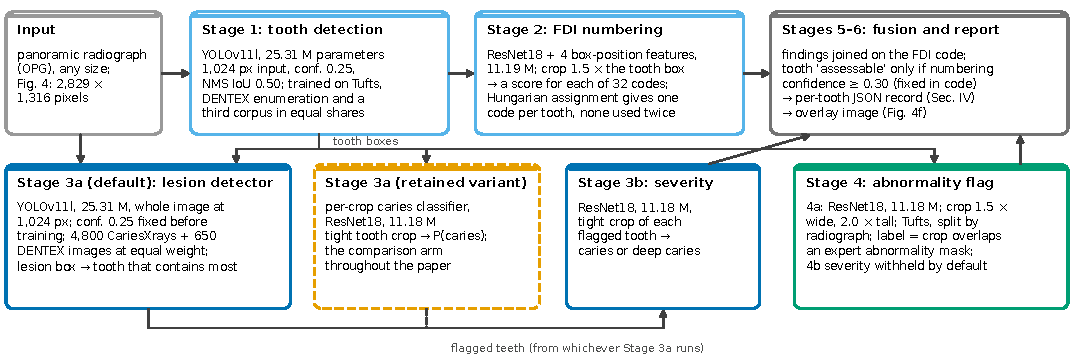
\includegraphics[width=0.90\textwidth]{figures/R06_architecture.pdf}
\caption{The pipeline as it ships, with its default checkpoints and learnable parameter counts read from the saved weights. Blue: identity stages; dark blue: the default caries path; dashed orange: the retained crop classifier, the comparison arm throughout; green: the abnormality flag. Thresholds are fixed in code; none was tuned on an evaluation cohort.}
\label{fig:3}
\end{figure*}

Fig.~\ref{fig:4} follows one held-out radiograph through every stage. For tooth 36 the record holds the code (confidence 0.9999), detection confidence 0.8389, a deep-caries finding (caries confidence 0.8892, severity 0.9579), no Stage-4 flag (0.7853) and an assessability flag.

\begin{figure*}[t]
\centering
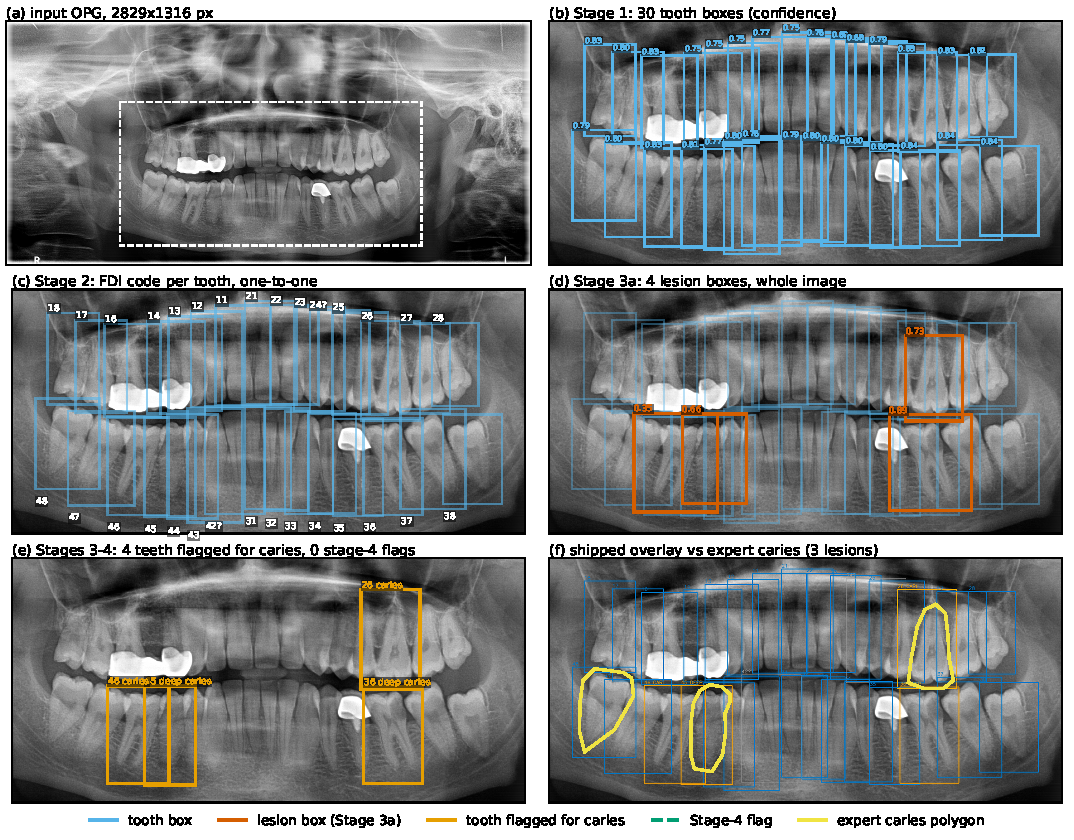
\includegraphics[width=0.92\textwidth]{figures/R02_walkthrough.pdf}
\caption{One held-out DENTEX radiograph (test\_0, not used to train any model) through the shipped pipeline. (a) Input; dashed: the region shown in (b)-(f). (b) Stage 1: 30 teeth, with detection confidences. (c) Stage 2: one FDI code per tooth; "?" marks two unsure codes. (d) Stage 3a: one lesion-detector pass over the whole image, four boxes. (e) Each box goes to the tooth holding most of it: 26 and 46 flagged as caries, 36 and 45 as deep caries. (f) The written overlay with the expert's three caries annotations (26, 45, 48) in yellow: two found, 48 missed, 36 flagged with no annotated lesion. Radiograph: DENTEX~\cite{hamamci2023dentex}, CC BY-NC-SA 4.0.}
\label{fig:4}
\end{figure*}

\section{Data and Evaluation Protocol}

\textbf{Cohorts and exposure.} Table~\ref{tab:2} lists every evaluation population and which model saw it. All splits are by image. DENTEX's disease subset has 250 annotated radiographs; MD5 hashing found 86 byte-identical to images our models trained on, leaving 164 scored, of which 148 carry a caries lesion. A perceptual-hash search against the 1,389 other DENTEX images found no further copy: the 86 lie at distance 0, and the 20 scored images nearest to them differ in restorations or missing teeth. The Ningxia public release divides its test data into four sets, one from its training centre and three described as cross-centre; the source paper describes three hospitals~\cite{li2024multicenter}, and we treat the four sets as four sites.

\begin{table*}[t]
\centering
\caption{Evaluation cohorts, units and exposure. Each row is an analysis population; counts must not be summed across rows.}
\label{tab:2}
\footnotesize
\setlength{\tabcolsep}{3pt}
\begin{tabular}{>{\raggedright\arraybackslash}p{2.20cm}r>{\raggedright\arraybackslash}p{4.37cm}>{\raggedright\arraybackslash}p{9.07cm}}
\toprule
Cohort & Images & Unit (n) & Role and exposure \\
\midrule
DENTEX disease & 164 & 936 teeth; 477 carious; 479 lesions & development: the tooth detector trained on other DENTEX images; the lesion detector on DENTEX caries boxes \\
Ningxia, 4 sites & 337 & 1,013 lesions & external: never trained on; informed the lesion detector's adoption \\
CariesXrays & 1,200 & 2,815 lesions & external for the crop classifier; the lesion detector's validation split \\
Tufts test & 143 & 3,760 teeth (numbering); 3,892 (Stage 4) & both trained on the Tufts training split \\
UFBA-425 & 425 & 11,591 teeth & numbering only; no model trained on it \\
\bottomrule
\end{tabular}
\end{table*}

\textbf{Systems compared.} Four systems answer one question, which teeth in this radiograph show caries, on the same 164 images: the pipeline (with each Stage-3a implementation), Qwen2.5-VL-32B and Qwen2.5-VL-7B~\cite{bai2025qwen25vl}, both zero-shot with the FDI scheme in the prompt, and the constant of Section III-B. The language models were also shown a blank grey image and a random-noise image as content-free controls.

\textbf{Metrics and statistics.} FDI-set F1 (2) is micro-averaged over teeth. Lesion agreement (4) matches each expert lesion to a flagged tooth, by centroid containment on the external cohorts and by greedy intersection over union of at least 0.30 with a centroid fallback on DENTEX; every comparison is therefore within a cohort. Teeth in one radiograph share exposure, anatomy and annotator, so we resample images, not teeth~\cite{field2007bootstrapping}: intervals are 95\% percentile cluster bootstraps over images, 10,000 resamples with seed 42, except 2,000 for the crop classifier's calibration, 5,000 for its within-type AUC and 1,000 with seed 0 for the two abstention gains. Differences are system minus comparator in percentage points (pp), recomputed on each resample of the shared images. Across sites we pool the per-site differences by DerSimonian-Laird random effects~\cite{dersimonian1986meta} and report $I^2$~\cite{higgins2002quantifying}, the prediction interval for a new site~\cite{riley2011interpretation}, the Hartung-Knapp-Sidik-Jonkman interval, which suits few sites better~\cite{inthout2014hartung}, and a Q-profile interval for the between-site deviation $\tau$~\cite{viechtbauer2007confidence}. We report estimates with intervals, not a family of tests, and apply no multiplicity correction.

\textbf{What was fixed in advance, and what was not.} The lesion detector's adoption rule was committed before any arm was trained, so that the comparison with the constant could not be tuned after the fact: lesion agreement above both the constant's and the crop classifier's on at least two of three cohorts, with a rate of flagged teeth no more than 1.5 times the constant's on those cohorts. The tooth detector was different. It missed its pre-registered guard on the Tufts test split, box mAP@0.5 0.587 against 0.723 for a Tufts-only control, and was adopted by a dated decision for its numbering and caries behaviour. We report that decision as one taken against the registered rule, because the credibility of this evaluation rests on reporting registered outcomes as they fell.

\section{Results}

\subsection{RQ1: does the score separate a pipeline from the image-blind list?}

\textbf{On development data both pipelines lead and both language models fall below.} Table~\ref{tab:3} gives the four systems on the 164 DENTEX images. The pipeline with the lesion detector scores F1 0.498, 17.80 points above the constant [+13.48, +22.02], and is the only system with precision well above the constant's (0.439 against 0.218). The pipeline with the crop classifier leads by 4.27 points [+1.58, +7.05] at barely higher precision. Both language models see the radiograph and score below the list that does not: by 7.32 points for the 32B model and 17.04 for the 7B, both intervals excluding zero. Fig.~\ref{fig:5} places each system against the image-blind list at its own volume. Volume explains neither pipeline lead: against an image-blind answer that names as many codes, the leads are +22.35 [+17.42, +27.18] and +5.50 [+2.84, +8.22], while the language models are level with lists of their own size. Shown no anatomy, the smaller model returned the same two teeth for a blank image, for noise and for one of the two real radiographs on record, and the larger one answered noise with exactly the constant's eight molars. None of this is yet evidence of perception, because the tooth detector trained on this corpus.

\begin{table}[t]
\centering
\caption{Tooth-level caries prediction on 164 DENTEX images (477 carious teeth), micro-averaged. P: precision; R: recall; Matched: F1 minus that of an image-blind answer naming as many codes (pp).}
\label{tab:3}
\footnotesize
\setlength{\tabcolsep}{3pt}
\begin{tabular}{>{\raggedright\arraybackslash}p{3.82cm}rrrr}
\toprule
System & P & R & F1 & Matched \\
\midrule
Pipeline, lesion detector & 0.439 & 0.574 & 0.498 & +22.35 \\
Pipeline, crop classifier & 0.237 & 0.765 & 0.362 & +5.50 \\
Constant (image-blind) & 0.218 & 0.600 & 0.320 & — \\
Qwen2.5-VL-32B, zero-shot & 0.250 & 0.243 & 0.246 & +0.39 \\
Qwen2.5-VL-7B, zero-shot & 0.248 & 0.107 & 0.149 & +1.39 \\
Constant fitted on the scored images & 0.245 & 0.505 & 0.330 & — \\
\bottomrule
\end{tabular}
\end{table}

\begin{figure}[t]
\centering
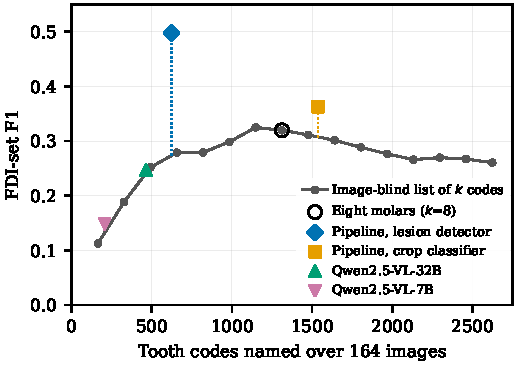
\includegraphics[width=0.98\columnwidth]{figures/V2_operating_curve.pdf}
\caption{The image-blind operating curve on the 164 DENTEX images. Grey: F1 of the $k$ most prevalent fit-set codes, $k$ = 1 to 16, against the number of codes named; circle: the eight-molar list. Each system is placed at its own volume; a dotted line drops to the matched image-blind answer. The lesion detector sits above the curve and names fewer codes than the molar list; the language models sit on it.}
\label{fig:5}
\end{figure}

\textbf{On external data the crop classifier's lead disappears.} Under lesion agreement the crop classifier leads the constant on DENTEX by 17.12 points [+12.15, +21.89], partly by volume, since it flags 1,439 teeth against 988. On the four Ningxia sites pooled, the two are level, 0.600 against 0.591, a difference of +0.89 points [$-$3.86, +5.57] (Table~\ref{tab:4}). On CariesXrays the constant leads, 0.604 against 0.379 ($-$22.42 [$-$24.62, $-$20.18]), while flagging more teeth at a higher match rate, so volume does not explain it. Within the one external cohort, the difference runs from $-$18.99 [$-$26.32, $-$11.84] at test1 to +12.32 [+5.01, +19.20] at test2, a 31-point swing, while the constant's own agreement, each site's prior mass on the eight molars, ranges from 0.494 to 0.709 (Fig.~\ref{fig:6}). Outside the corpus its tooth detector trained on, the classifier's lead is not consistent: it trails the constant at one site, leads at another, and is level when the sites are pooled. This tie on external data would also be expected from ordinary domain shift with no positional prior at all; the next analysis asks whether the classifier has in fact absorbed the prior.

\begin{table*}[t]
\centering
\caption{Lesion agreement of the three caries options under the current tooth detector, with the number of teeth flagged; last columns, paired differences (pp, 95\% CI). CariesXrays is the lesion detector's validation split.}
\label{tab:4}
\footnotesize
\setlength{\tabcolsep}{3pt}
\begin{tabular}{>{\raggedright\arraybackslash}p{3.07cm}>{\raggedright\arraybackslash}p{2.25cm}>{\raggedright\arraybackslash}p{1.70cm}>{\raggedright\arraybackslash}p{2.25cm}rr}
\toprule
Cohort & Crop classifier & Constant & Lesion detector & Classifier minus constant & Detector minus constant \\
\midrule
DENTEX (164) & 0.802 (1,439) & 0.630 (988) & 0.595 (603) & +17.12 [+12.15, +21.89] & $-$3.55 [$-$10.11, +2.64] \\
CariesXrays (1,200) & 0.379 & 0.604 & 0.757 & $-$22.42 [$-$24.62, $-$20.18] & +15.38 [+12.96, +17.73] \\
Ningxia, pooled (337) & 0.600 & 0.591 & 0.684 & +0.89 [$-$3.86, +5.57] & +9.28 [+4.72, +13.73] \\
\bottomrule
\end{tabular}
\end{table*}

\textbf{The classifier's scores follow position, and its ranking still carries image signal.} Table~\ref{tab:5} applies the test of Section III-E to 863 held-out tooth crops from 34 radiographs, cut with ground-truth boxes so that the front end plays no part. The classifier's mean score on truly healthy teeth climbs with the training base rate, from 0.075 on incisors to 0.478 on molars, and it flags 48.2\% of healthy molars: the prior is doing visible work, and costs precision. Its within-type AUC is 0.745 [0.660, 0.842], so genuine lesion signal remains, and its average precision (AP) of 0.550 is above that of a predictor using position alone (0.296) and chance (0.147). The classifier is neither a lookup table nor a pure reader, but a reader whose score is inflated by a prior the constant captures for free.

\begin{table*}[t]
\centering
\caption{The positional-shortcut test on the crop classifier: 863 held-out crops from 34 radiographs. Base rate: share carious in its training data. Interval: cluster bootstrap over the 34 radiographs, 5,000 resamples.}
\label{tab:5}
\footnotesize
\setlength{\tabcolsep}{3pt}
\begin{tabular}{>{\raggedright\arraybackslash}p{5.06cm}rrrrrr}
\toprule
Tooth type & Crops & Carious & Base rate & Mean score, healthy & Healthy flagged & Within-type AUC \\
\midrule
Incisor & 266 & 8 & 0.017 & 0.075 & 0.039 & 0.681 \\
Canine & 129 & 5 & 0.023 & 0.087 & 0.016 & 0.748 \\
Premolar & 221 & 31 & 0.157 & 0.273 & 0.268 & 0.782 \\
Molar & 247 & 83 & 0.343 & 0.478 & 0.482 & 0.781 \\
All, within type & 863 & 127 & — & — & — & 0.745 [0.660, 0.842] \\
\bottomrule
\end{tabular}
\end{table*}

Direct repairs of the classifier came first. Three were run against a same-day control under a rule fixed in advance: contrast equalisation, a crop widened 1.25 times and position-balanced sampling. An earlier retrain with 2.67 times the carious crops was compared against the shipped model. None separated from zero; the largest, contrast equalisation, changed AP by +0.049 [$-$0.003, +0.099], and the retrain by $-$0.0015 [$-$0.0886, +0.0821]. With 34 source radiographs these comparisons have little power, but a retrain with nearly three times the positives also did nothing, which points at the task as posed rather than at the supervision. We therefore changed the task.

\subsection{RQ2: does localising lesions separate the pipeline from the list?}

\textbf{The lesion detector met its registered rule and leads on the external sites with fewer flags.} Under the tooth detector of the time, the lesion detector met the adoption rule on CariesXrays and Ningxia and tied on DENTEX. Under the current tooth detector (Table~\ref{tab:4}) it leads the constant on the four Ningxia sites pooled by 9.28 points [+4.72, +13.73], 0.684 against 0.591, and on CariesXrays by 15.38 [+12.96, +17.73], while it is not separated from the constant on DENTEX ($-$3.55 [$-$10.11, +2.64]). It flags 4.35 teeth per image against the constant's 7.15 on Ningxia, and 2.16 against 7.05 on CariesXrays, so neither lead is bought with volume. The Ningxia lead is the external one: CariesXrays is the split on which the detector's checkpoint was chosen. On DENTEX the retired crop classifier scores higher on agreement (0.802 against 0.595) by flagging 2.4 times as many teeth; F1, which charges for false positives, orders the two the other way round (0.498 against 0.362).

\begin{figure}[t]
\centering
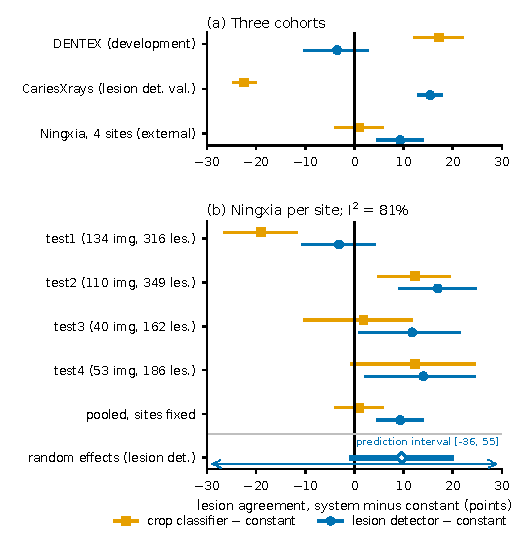
\includegraphics[width=0.98\columnwidth]{figures/R07_paired_differences.pdf}
\caption{Lesion agreement of each caries option minus the constant, paired 95\% cluster-bootstrap intervals (10,000 resamples). (a) Per cohort; DENTEX is development data for the front end, and CariesXrays is the lesion detector's validation split. (b) The four Ningxia sites, the pooled difference with sites fixed, and the random-effects mean for the lesion detector (diamond; bar: 95\% interval; dotted, beyond the axis: prediction interval for a new site).}
\label{fig:6}
\end{figure}

\textbf{The lead holds at three of four sites and is not shown for an unseen site.} Per site (Fig.~\ref{fig:6}(b)) the lesion detector is separated from the constant at test2, test3 and test4 (+16.91 [+9.17, +24.62], +11.73 [+1.07, +21.34], +13.98 [+2.34, +24.34]) and not at test1 ($-$3.16 [$-$10.56, +3.97]), where the constant is strongest. Treating the sites as a sample (random effects, post hoc) gives +9.61 [$-$0.54, +19.76] (Hartung-Knapp [$-$5.02, +24.24]), $I^2$ 81\%, $\tau$ 9.27 points [3.22, 33.09] and a prediction interval of [$-$36.08, +55.29]. With four sites the between-site deviation could lie anywhere from about 3 to 33 points, so the lead holds at these sites and is not shown for a new one. Ningxia also informed the detector's adoption, so this lead is optimistic by construction.

\textbf{What supports reading the image, and what does not.} Both implications of Section III-F are observed. The lead comes with fewer flags, and on DENTEX, the only cohort with per-tooth records, the detector's flags are carious more often within each tooth type: 46.3\% of the molars it flags carry caries, against 28.4\% for the crop classifier and 21.8\% for the constant, and 39.7\% of its flagged premolars against 17.0\%. Two things argue for caution. The per-type comparison is not available on the external cohort, whose saved outputs hold per-image counts only. And the change of task came with new training data: under the tooth detector of the time, the same detector trained on CariesXrays alone reached 0.694 [0.674, 0.714] on CariesXrays and collapsed to 0.086 [0.055, 0.119] on DENTEX and 0.240 [0.209, 0.272] on Ningxia, so the training mixture, not the architecture, is what transferred. Fig.~\ref{fig:7} shows the range on three images chosen by a rule fixed before rendering: all seven lesions found, two of three, and none of four.

\begin{figure*}[t]
\centering
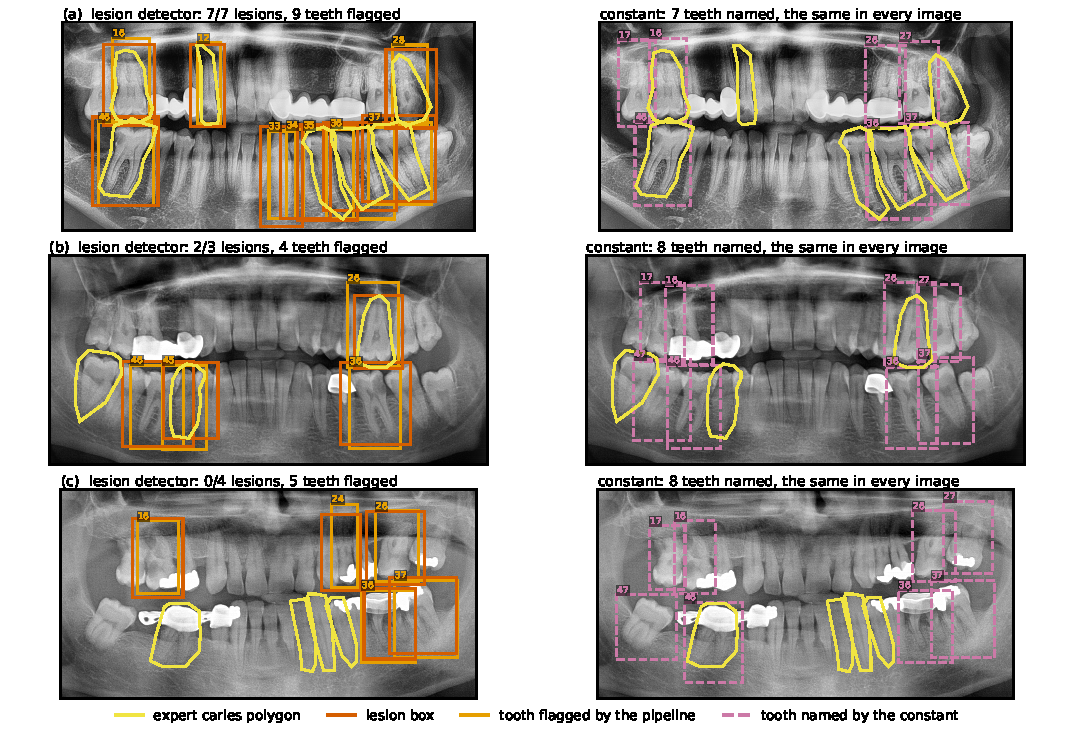
\includegraphics[width=0.90\textwidth]{figures/R03_outcomes.pdf}
\caption{Pipeline output against the expert on three held-out DENTEX radiographs, chosen by a rule fixed before rendering (the scored image with the most lesions all found, a typical image, the image with the most lesions none found). Left: the lesion detector; right: the constant placed by the same front end. (a) test\_120: all seven lesions found, 33 and 34 also flagged; the constant covers four of the seven without reading the image. (b) test\_0 (Fig.~\ref{fig:4}): two of three found, 48 missed. (c) test\_110: none of four found. A flag without an annotated lesion is not a confirmed false positive: the exhaustiveness of the annotation is not documented. Radiographs: DENTEX~\cite{hamamci2023dentex}, CC BY-NC-SA 4.0.}
\label{fig:7}
\end{figure*}

\subsection{RQ3: what the pipeline shows that a list cannot}

\textbf{Identity.} End-to-end FDI-exact accuracy is 92.8\% on DENTEX, an in-domain figure, and 44.5\% on UFBA-425, which no model trained on (Table~\ref{tab:1}). Of 63 wrong codes on DENTEX, 51 name an adjacent tooth in the correct quadrant, and only 6 of 932 detected teeth get a quadrant-level error. At molar positions, where most caries lies, 8.2\% of detected second molars receive a wrong code, and each such error moves any finding to the wrong tooth: the second factor of (1). The constant in our agreement tables is placed by this same front end, which missed its registered Tufts guard.

\textbf{Selective prediction and calibration.} Declining the least-confident quarter raises numbering accuracy from 0.932 to 0.980 (+4.76 points [+3.29, +6.54]) and the crop classifier's from 0.797 to 0.940 (+14.25 [+11.32, +16.63]); with confidences shuffled across items both gains vanish, to $-$0.06 and +0.00 points, so the gain comes from the ranking and not from discarding items~\cite{geifman2017selective}. Calibration is measured on the crop classifier, because the lesion detector emits detection scores rather than per-tooth probabilities. The classifier is overconfident: at a stated confidence of 0.85 the observed share carious is 0.26, and its expected calibration error~\cite{naeini2015obtaining,guo2017calibration} is 0.136. Temperature scaling made it worse (0.152); isotonic regression~\cite{zadrozny2002isotonic} reduced it to 0.043 at a cost in AP (0.550 to 0.500), so it adjusts only the reported confidence. Fig.~\ref{fig:8} collects these outputs.

\begin{figure*}[t]
\centering
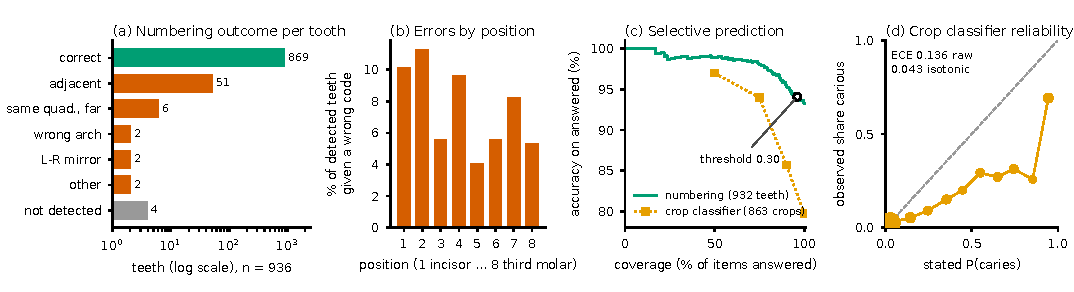
\includegraphics[width=0.86\textwidth]{figures/R08_numbering_reliability.pdf}
\caption{Outputs a fixed list cannot produce. (a) Numbering outcome for each of 936 ground-truth DENTEX teeth (log scale). (b) Share of detected teeth given a wrong code, by position. (c) Accuracy on the items answered as the least confident are declined: numbering, from saved per-tooth confidences (circle: the 0.30 threshold fixed in code); crop classifier, saved operating points. (d) Reliability of the crop classifier's raw confidence on 863 held-out crops (marker area proportional to bin count).}
\label{fig:8}
\end{figure*}

\textbf{A second branch shows the same lesson about measurement.} The abnormality flag's first model reported macro-F1 0.923 on a split that let every validation radiograph also supply training crops. Held out, it found 7.6\% of its labelled teeth, and 6 of 175 on the Tufts test radiographs it had not seen. Retrained with a radiograph-level split, three runs found 27.5\%, 16.5\% and 11.0\% (50, 30 and 20 of 182) on 143 held-out radiographs. Its severity head, retrained on bands of mask overlap, did not meet its registered rule against an image-blind tooth-position prior: the registered run scored macro-F1 0.294 [0.214, 0.385] against the prior's 0.334, and two further runs scored 0.328 and 0.382. The head stays withheld. A figure that looked like validation was a property of the split, as the caries scores of Section VI-A were partly a property of the prior.

\section{Discussion}

\subsection{Answers to the three questions}

\textbf{RQ1.} No, not by itself. The same metric moved by about 40 points across cohorts and by 31 within one cohort's sites, and a classifier that led the image-blind list on development data was level with it externally. On these cohorts a favourable tooth-level figure on development data was weak evidence of perception.

\textbf{RQ2.} Partly. A detector that must place lesion boxes can express a positional prior only at a cost in precision. It led the list on the pooled external sites with fewer flags, and on development data its flags were carious more often within each tooth type. This is consistent with reading the image, but the change of task is confounded with new training data, Ningxia informed the adoption, the site-level interval includes zero, and test1, where the constant is strongest, remains unexplained.

\textbf{RQ3.} Numbering, calibration and shuffle-controlled abstention are outputs a fixed list cannot attempt. They show confidence that ranks the system's own errors.

\subsection{How far the account holds}

Table~\ref{tab:6} sets each implication of Section III against the measurements. Because the account was written afterwards, this is a consistency check. Four implications hold, the localisation one only at three of four sites. One holds without singling out the account, because ordinary domain shift predicts it too. One is not supported: the prior inflates the classifier's thresholded scores, but its ranking within a tooth type carries real image signal.

\begin{table*}[t]
\centering
\caption{What the account of Section III implies, and what the measurements show (post hoc).}
\label{tab:6}
\footnotesize
\setlength{\tabcolsep}{3pt}
\begin{tabular}{>{\raggedright\arraybackslash}p{4.10cm}>{\raggedright\arraybackslash}p{8.36cm}>{\raggedright\arraybackslash}p{4.27cm}}
\toprule
Implication & Evidence & Verdict \\
\midrule
Rule (3) gives the best constant & reproduces the fitted eight molars; recall 0.600 = carious share at them & holds \\
The floor moves with the cohort & the constant's agreement ranges 0.494 to 0.709 across four sites & holds \\
A shortcut lifts healthy scores & healthy score 0.075 (incisors) to 0.478 (molars); 48.2\% of healthy molars flagged & holds \\
A shortcut carries the ranking & within-type AUC 0.745 [0.660, 0.842] & not supported \\
Agreement does not transfer & classifier minus constant +17.12, +0.89, $-$22.42 on the three cohorts & holds; also expected from domain shift \\
Localising gives fewer, better flags & Ningxia +9.28 with 4.35 vs 7.15 flags per image; DENTEX flagged molars 46.3\% vs 28.4\% carious & 3 of 4 sites \\
\bottomrule
\end{tabular}
\end{table*}

\subsection{What a paper should report with a tooth-level caries score}

Our results suggest that a tooth-level caries score should not travel alone. Table~\ref{tab:7} lists what we recommend reporting beside it, complementing the general and dental reporting checklists~\cite{mongan2020claim,schwendicke2021checklist}.

\begin{table}[t]
\centering
\caption{What to report with a tooth-level caries score.}
\label{tab:7}
\footnotesize
\setlength{\tabcolsep}{3pt}
\begin{tabular}{>{\raggedright\arraybackslash}p{4.73cm}>{\raggedright\arraybackslash}p{3.03cm}}
\toprule
Item & Why \\
\midrule
An image-blind constant fitted off the test set, with rule (3) & sets the floor the metric allows without an image \\
A matched-volume constant for each system & separates a lead from naming more teeth \\
The identity factors: detection and numbering accuracy & bound every finding attached to a tooth code \\
Per-site external results with paired intervals, and a random-effects prediction interval & a pooled lead can hide sites where it fails \\
Flag counts, and images chosen by a stated rule & agreement has no negative class \\
\bottomrule
\end{tabular}
\end{table}

\section{Limitations}

The authors' own limitations come first; each bounds named claims.

\begin{itemize}
\item DENTEX is in-domain for the tooth detector, which missed its Tufts guard (0.587 against 0.723). Only Ningxia is external to the lesion detector, it informed the adoption, and the random-effects interval includes zero. The development-data leads are weak evidence of perception, and the external lead is optimistic by construction.
\item The account treats codes independently and was checked on one corpus (78 and 164 images); the shortcut test rests on 34 radiographs; the lesion detector has no calibration curve. The floor's value is specific to this corpus's prior.
\item DENTEX caries labels were read from panoramic radiographs alone, which detect proximal caries less accurately than bitewings~\cite{akarslan2008comparison}. The expert lesions are a subset of disease, and part of the molar prior may be a prior of what panoramic labels capture.
\item Agreement has no negative class and the external cohorts no healthy controls, so no false-positive rate can be given; every model except Stage 4 is a single training run, so intervals cover the sampling of images only; no clinician comparison was made; and duplicate checks cannot find a patient's second radiograph.
\item The CariesXrays images are the lesion detector's validation split, split by image while some patients have several images, so its CariesXrays figure is a validation-split figure; Ningxia is the only cohort the lesion detector neither trained nor selected on.
\item The constant in the agreement tables is placed by the pipeline's own boxes and numbering, and numbering on unseen data is low (44.5\%); the scored DENTEX images hold no tooth labelled healthy.
\item The abnormality flag's severity head was first trained on image contrast instead of mask overlap, and the flag's sensitivity depends on the training run; no severity or periodontal claim is made.
\item Per-tooth-type precision is shown on development data only, the duplicate checks find copies and not patients, and the constant's exact membership is unstable: the floor's score, not its set, is what should be cited.
\item The figures show DENTEX radiographs under a share-alike licence; the adoption rule's registration is in a private history with no public anchor; the language models' decoding settings and the CPU behind the runtime are not recorded; the statement about the dental papers we surveyed is an observation, not a count; and the Ningxia source paper describes three hospitals while its release has four test sets.
\end{itemize}

Additional caveats. The account of Section III was written after the measurements it explains, so its agreement with them is a consistency check only. The runtime has two records (1.70 s and 1.37 s per image) and no recorded processor, and two runs of the smaller language model differ slightly (F1 0.143 and 0.149).

\section{Conclusion}

A tooth-level caries score mixes what a system sees with where caries usually is. The image-blind part has a closed form; here it is the eight first and second molars, at F1 0.320. A crop classifier sat above that floor on its development data and level with it at four external sites, while a lesion detector led it there with fewer flags, at three of the four. Because the floor differs between populations and sites, the score should travel with an image-blind row, per-site results and outputs a fixed list cannot produce. Four checks remain open: the per-tooth-type comparison on external data, a learned position-only floor, a content ablation that blurs tooth interiors, and a probe of whether images reveal their site.

\section*{Data and Code Availability}

[ASK AUTHOR: code, weights and data availability statement; DENTEX is CC BY-NC-SA 4.0, the Tufts images may not be redistributed]

\section*{Acknowledgment}

[ASK AUTHOR: acknowledgment and AI-use wording; a draft is in disclosure.md]

\bibliographystyle{IEEEtran}
\bibliography{references}
\end{document}
